%%%%%%%%%%%%%%%%%%%%%%%%%%%%%%%%%%%%%%%%%
% kaobook
% LaTeX Class
% Version 0.9.8 (2021/08/23)
%
% This template originates from:
% https://www.LaTeXTemplates.com
%
% For the latest template development version and to make contributions:
% https://github.com/fmarotta/kaobook
%
% Authors:
% Federico Marotta (federicomarotta@mail.com)
% Based on the doctoral thesis of Ken Arroyo Ohori (https://3d.bk.tudelft.nl/ken/en)
% and on the Tufte-LaTeX class.
% Modified for LaTeX Templates by Vel (vel@latextemplates.com)
%
% License:
% LPPL (see included MANIFEST.md file)
%
%%%%%%%%%%%%%%%%%%%%%%%%%%%%%%%%%%%%%%%%%

%----------------------------------------------------------------------------------------
%	EXAMPLE AND DOCUMENTATION OF THE KAOBOOK CLASS
%----------------------------------------------------------------------------------------

\documentclass[
    letterpaper, % Page size
    fontsize=10pt, % Base font size
    twoside=false, % Use different layouts for even and odd pages (in particular, if twoside=true, the margin column will be always on the outside)
	%open=any, % If twoside=true, uncomment this to force new chapters to start on any page, not only on right (odd) pages
	%chapterentrydots=true, % Uncomment to output dots from the chapter name to the page number in the table of contents
	numbers=noenddot, % Comment to output dots after chapter numbers; the most common values for this option are: enddot, noenddot and auto (see the KOMAScript documentation for an in-depth explanation)
]{kaobook}

%----------------------------------------------------------------------------------------
%	PACKAGES AND OTHER DOCUMENT CONFIGURATIONS
%----------------------------------------------------------------------------------------

% Choose the language
\ifxetexorluatex
	\usepackage{polyglossia}
	\setmainlanguage{english}
\else
	\usepackage[english]{babel} % Load characters and hyphenation
\fi
\usepackage[english=british]{csquotes}	% English quotes

% Load packages for testing
\usepackage{blindtext} % Print text without any meaning for testing purposes
%\usepackage{showframe} % Uncomment to show boxes around the text area, margin, header and footer
%\usepackage{showlabels} % Uncomment to output the content of \label commands to the document where they are used

% Load the bibliography package
\usepackage{kaobiblio}
\addbibresource{main.bib} % Bibliography file

% Load mathematical packages for theorems and related environments
\usepackage[framed=true]{kaotheorems}

% Load the package for hyperreferences
\usepackage{kaorefs}

\graphicspath{{examples/documentation/images/}{images/}} % Paths in which to look for images

\makeindex[columns=3, title=Alphabetical Index, intoc] % Make LaTeX produce the files required to compile the index

\makeglossaries % Make LaTeX produce the files required to compile the glossary
\newglossaryentry{computer}{
	name=computer,
	description={is a programmable machine that receives input, stores and manipulates data, and provides output in a useful format}
}

% Glossary entries (used in text with e.g. \acrfull{fpsLabel} or \acrshort{fpsLabel})
\newacronym[longplural={Frames per Second}]{fpsLabel}{FPS}{Frame per Second}
\newacronym[longplural={Tables of Contents}]{tocLabel}{TOC}{Table of Contents}

 % Include the glossary definitions

\makenomenclature % Make LaTeX produce the files required to compile the nomenclature

% Reset sidenote counter at chapters
%\counterwithin*{sidenote}{chapter}

%----------------------------------------------------------------------------------------

\begin{document}

%----------------------------------------------------------------------------------------
%	BOOK INFORMATION
%----------------------------------------------------------------------------------------


\title[ Full Self-Driving, Skynet and other Artificial Intelligence Myths ]{ Full Self-Driving Skynet, and Other Artificial Intelligence Myths }
\subtitle{ The realities of decision making with deep machine learning models }

\author[Brad Flaugher]{Brad Flaugher}

\date{\today}

\publishers{}

%----------------------------------------------------------------------------------------

\frontmatter % Denotes the start of the pre-document content, uses roman numerals

%----------------------------------------------------------------------------------------
%	OPENING PAGE
%----------------------------------------------------------------------------------------

%\makeatletter
%\extratitle{
%	% In the title page, the title is vspaced by 9.5\baselineskip
%	\vspace*{9\baselineskip}
%	\vspace*{\parskip}
%	\begin{center}
%		% In the title page, \huge is set after the komafont for title
%		\usekomafont{title}\huge\@title
%	\end{center}
%}
%\makeatother

%----------------------------------------------------------------------------------------
%	COPYRIGHT PAGE
%----------------------------------------------------------------------------------------

\makeatletter
\uppertitleback{\@titlehead} % Header

\lowertitleback{
	\textbf{Disclaimer}\\
	You can edit this page to suit your needs. For instance, here we have a no copyright statement, a colophon and some other information. This page is based on the corresponding page of Ken Arroyo Ohori's thesis, with minimal changes.
	
	\medskip
	
	\textbf{No copyright}\\
	\cczero\ This book is released into the public domain using the CC0 code. To the extent possible under law, I waive all copyright and related or neighbouring rights to this work.
	
	To view a copy of the CC0 code, visit: \\\url{http://creativecommons.org/publicdomain/zero/1.0/}
	
	\medskip
	
	\textbf{Colophon} \\
	This document was typeset with the help of \href{https://sourceforge.net/projects/koma-script/}{\KOMAScript} and \href{https://www.latex-project.org/}{\LaTeX} using the \href{https://github.com/fmarotta/kaobook/}{kaobook} class.
	
	The source code of this book is available at:\\\url{https://github.com/fmarotta/kaobook}
	
	(You are welcome to contribute!)
	
	\medskip
	
	\textbf{Publisher} \\
	First printed in May 2019 by \@publishers
}
\makeatother

%----------------------------------------------------------------------------------------
%	DEDICATION
%----------------------------------------------------------------------------------------

\dedication{
	We have now accumulated sufficient evidence to see that whatever language the central nervous system is using, it is characterized by less logical and arithmetical depth than what we are normally used to.\\
	-- John von Neumann \cite{vonNeumann2012}
}

%----------------------------------------------------------------------------------------
%	OUTPUT TITLE PAGE AND PREVIOUS
%----------------------------------------------------------------------------------------

% Note that \maketitle outputs the pages before here

\maketitle

%----------------------------------------------------------------------------------------
%	PREFACE
%----------------------------------------------------------------------------------------

\chapter*{Preface}
\addcontentsline{toc}{chapter}{Preface} % Add the preface to the table of contents as a chapter

This book is a work in progress, I hope it helps demystify the world of deep learning as I understand it.

Humans won't be able to control superintelligent AI, talk about that here\cite{Andreu2021}

Talk about Bostrom and GPAI here, and Erdi's answer to that. \cite{Erdi2019} \cite{Bostrom2014}

Talk about the alignment problem and Ethical freakouts about AI. Talk about the big 3 from 
\cite{Christian2020}
\cite{Blackman2022Jul}

Funding and startups, everybody is doing it, I'm trying to make sense of it


\begin{flushright}
	\textit{Brad Flaugher}
\end{flushright}

\index{preface}

%----------------------------------------------------------------------------------------
%	TABLE OF CONTENTS & LIST OF FIGURES/TABLES
%----------------------------------------------------------------------------------------

\begingroup % Local scope for the following commands

% Define the style for the TOC, LOF, and LOT
%\setstretch{1} % Uncomment to modify line spacing in the ToC
%\hypersetup{linkcolor=blue} % Uncomment to set the colour of links in the ToC
\setlength{\textheight}{230\hscale} % Manually adjust the height of the ToC pages

% Turn on compatibility mode for the etoc package
\etocstandarddisplaystyle % "toc display" as if etoc was not loaded
\etocstandardlines % "toc lines as if etoc was not loaded

\tableofcontents % Output the table of contents

\listoffigures % Output the list of figures

% Comment both of the following lines to have the LOF and the LOT on 
% different pages
\let\cleardoublepage\bigskip
\let\clearpage\bigskip

\listoftables % Output the list of tables

\listoflstlistings % Output the list of listings

\endgroup

%----------------------------------------------------------------------------------------
%	MAIN BODY
%----------------------------------------------------------------------------------------

\mainmatter % Denotes the start of the main document content, resets page numbering and uses arabic numbers
\setchapterstyle{kao} % Choose the default chapter heading style

\setchapterpreamble[u]{\margintoc}
\chapter{Playing chess in 1997}
\labch{intro}

\section{"Textbook" AI in 1997}

Dr. Elaine Rich's textbook on Artificial Intelligence, published in the 1980s, was a groundbreaking work that helped to establish many of the foundational concepts and techniques in the field of AI. However, the rapid advancements in AI over the past few decades have led to many of the chapters in this textbook becoming obsolete.

One of the main reasons for this is the prevalence of deep learning, big data, and large-scale statistical models in modern AI. These techniques have largely replaced the symbolic, rule-based approach to AI that was emphasized in the textbook, making many of the chapters on knowledge representation and expert systems less relevant.

Additionally, the explosion of data and the availability of powerful computing resources have made it possible to apply machine learning techniques at a scale that was previously unimaginable. This has led to the development of highly effective machine learning models that can handle complex tasks such as image and speech recognition with a high degree of accuracy, making many of the chapters on simpler machine learning techniques such as decision trees\sidenote{Although mathematically, \href{https://arxiv.org/abs/2210.05189}{Neural Networks are Decision Trees}} and linear regression less relevant. \sidecite{rich_2009} \sidenote{the book is now in its third edition and unlikely to be updated as Dr. Rich as retired \href{https://www.cs.utexas.edu/~ear/}{utexas.edu}}


We'll discuss this history and a few examples from the "early days" of AI to help us understand where we are headed.

\section{Teaching computers to translate}

Noam Chomsky is a linguist and philosopher who has made significant contributions to the field of linguistics with his theory of universal grammar. Chomsky believes that all human languages share a common underlying structure, and that this structure is innate to humans. He proposes that this innate structure is the result of a "language acquisition device" present in the human brain, which allows us to learn and produce language. Chomsky also argues that the structure of language is largely independent of its content, and that the ability to produce and understand language is a fundamental aspect of human nature. His theory has been influential in the field of linguistics and has sparked much debate and research on the nature of language and its relationship to the human mind.

For English speakers or anyone who has learned English as a second language you'll have many examples of special cases, irregular verbs, bad english and former street slang that became good and proper over time. For programmers this is a nightmare, how can we codify human knowledge in a timely fashion? If we tried to write the rules of the english language in code (which many have tried to do) the rules themselves might change before we were finished writing them.

Explicitly translating languages through code is a difficult task because it requires a thorough understanding of the grammar, vocabulary, and syntax of both languages, as well as the nuances and subtleties of their respective cultures\sidenote{For programmers this is a nightmare, how can we codify human knowledge in a timely fashion? If we tried to write the rules of the english language in code (which many have tried to do) the rules themselves might change before we were finished writing them.}. Simply coding rules for how to translate words or phrases from one language to another is not sufficient, as there are often multiple valid translations for a given phrase depending on the context in which it is used.

A more effective approach to translation is to use statistical techniques that rely on a large corpus of translated data, such as Canadian laws. This type of data-driven approach involves training a machine learning model on a large dataset of translations, allowing it to learn the patterns and relationships between the languages. The model can then use this knowledge to make educated translations of new phrases or sentences, taking into account the context in which they are used.

While this approach is not perfect, it has proven to be highly effective in machine translation and can produce accurate translations even for languages that are very different from each other. The use of a large dataset of translations also allows the model to learn from the mistakes and variations present in real-world translations, further improving its accuracy.

\section{Codified human knowledge}

When we "teach" a computer to perform a task by explicitly writing down all of the rules of that task, we are really codifying human understanding.\sidenote{Programming this way makes some software development totally boring, I almost switched my major in college to math after considering what a life would look like manually writing rules for handling "edge cases" for the rest of my natural life.} When we codify human understanding we write down every rule that we know explicitly. For small tasks we can do this with 100 percent accuracy, and only minor headache on the part of the sofware developer. 

For example, let's write a boring function to tell you the number of days for a given month. 

\begin{lstlisting}[style=kaolstplain,linewidth=1.5\textwidth]
def days_in_month(year, month):
  if month in [1, 3, 5, 7, 8, 10, 12]:
    return 31
  elif month in [4, 6, 9, 11]:
    return 30
  elif month == 2:
    if (year % 4 == 0 and year % 100 != 0) or year % 400 == 0:
      return 29
    else:
      return 28
  else:
    return "Invalid month"

\end{lstlisting}

Writing code can be a tedious and repetitive task, especially when it comes to debugging and testing. It can be especially frustrating when you're working on a large project and you're trying to track down a specific bug that's causing the program to crash. Testing code can also be boring, as it often involves running the same tests over and over again to ensure that the code is working correctly.

Additionally, writing code can be boring because it requires a lot of concentration and focus. It can be easy to get lost in the details and lose track of time, especially if you're working on a complex problem. It can also be challenging to come up with creative solutions to problems, and it can be frustrating when your code doesn't work as expected.

While writing and testing code can be rewarding and fulfilling, it can also be a tedious and boring process. It requires a lot of patience, persistence, and attention to detail, and it can be easy to get frustrated and lose motivation. However, with practice and perseverance, it is possible to overcome these challenges and find enjoyment in the process of writing and testing code.

AI has traditionally operated by explicitly codifying human knowledge into machine-readable formats by doing the boring job of coding. This approach, which I'm calling "codified human knowledge" relies on humans to carefully structure and organize information in a way that can be understood by the AI system. The AI system then uses this structured knowledge to make decisions and perform tasks.

However, recent advances in AI have largely ignored the knowledge representation problem and instead have focused on using statistical techniques and neural networks to automatically learn patterns and relationships in data. This approach, known as "deep learning," involves training large neural networks on vast amounts of data, allowing the AI system to make educated classifications and transformations of data without explicit human guidance.

Deep learning has proven to be highly effective in a variety of applications, such as image and speech recognition, and has contributed to the rapid progress we have seen in AI in recent years. However, the reliance on large amounts of data and the lack of transparency in these models can make it difficult to understand how they are making decisions, which can be a concern in certain applications (hence the title of this book).

\section{Deep Blue's Brute Force Victory}

Deep Blue was a revolutionary computer developed by IBM that was specifically designed to play chess at the highest level. It was programmed with a vast database of chess knowledge and was able to analyze millions of positions per second.

Garry Kasparov was the reigning world chess champion at the time, and he was considered to be one of the greatest players in history. He had never lost a match to a computer before, and he was confident that he would be able to defeat Deep Blue.

However, things did not go as Kasparov had expected. Deep Blue was able to analyze the positions on the board with incredible speed and accuracy, and it was able to come up with highly sophisticated strategies that Kasparov had never seen before.

Despite Kasparov's best efforts, he was no match for the sheer brute force of Deep Blue's computational power. In the end, Deep Blue emerged victorious, defeating Kasparov in a historic match that changed the world of chess forever.

Deep Blue was a turning point in the development of AI, but Deep Blue's methods (namely calculating every possible outcome of a Chess game to determine the best move) was not suitable for many of the world's problems. It turns out that Chess is fun, but the world is not like chess. The "real" future of AI was being developed elsewhere, using statistics and a toy model of the brain to solve a very practical problem for banks.

\section{Meanwhile at the bank}

It was the early 1990s and Yann LeCun was a researcher at Bell Labs in New Jersey. At the time, the process of reading and processing checks was a tedious and time-consuming task that was done manually by bank employees. LeCun saw the potential for using artificial intelligence to automate this process, and he began experimenting with using convolutional neural networks (CNNs) to recognize patterns in images of checks.

At the time, CNNs were a relatively new type of neural network that had been developed in the 1980s for image recognition tasks. They were inspired by the structure of the human visual system, and were able to process images in a way that was similar to how the human brain does.

LeCun's work was groundbreaking, and he was able to achieve impressive results using CNNs to process checks. By 1993, he had developed a system that was able to read and process checks with a high degree of accuracy, significantly reducing the amount of time and effort that was required to process checks manually.

LeCun's work on using CNNs for check processing was a major milestone in the field of artificial intelligence, and it laid the foundation for the development of many other applications of CNNs in the years that followed. Today, CNNs are widely used in a variety of applications, including facial recognition, image classification, and natural language processing. \sidenote{check out Yann LeCun domonstrating a convolutional neural network in 1993 at \href{https://www.youtube.com/watch?v=FwFduRA_L6Q}{youtube.com}}

\section{Programmer intelligence, data intelligence and artificial intelligence}

I think it's useful to separate the actors in the AI problem-space into three groups. The data, the programmer and the machine learning (or AI) together they make the programs that we use every day, and for the rest of this book I'll try and separate the discussion of the smarts of each to help us better understand the world. \sidenote{I'll also repeatedly encourage you to use the words "algorithm" and "artificial intelligence" sparingly. They'll confuse your thinking, I promise.}

Programmer intelligence refers to the ability of a human programmer to design, write, and debug computer programs. This type of intelligence involves problem-solving skills, logical thinking, and the ability to learn and adapt to new programming languages and technologies. Most books don't talk about programmer intelligence and use the even more vague word "Algorithm" to describe both the programmer's output and the AI that might contibute to decision making, which can lead to misunderstanding.

Artificial intelligence is a terrible term. It generally refers to the ability of a machine or computer system to perform tasks that would normally require human intelligence, such as learning, problem-solving, and decision-making. Artificial intelligence systems can be trained to perform a wide range of tasks, from simple tasks like recognizing patterns in data to more complex tasks like understanding and generating natural language. Becuase the term is so broad I'll avoid it, and instead talk about machine learning and deep learning instead. \sidenote{In case I am confusing you, I think that Deep Blue was made with "Programmer Intelligence" or "Codified Human Knowledge" where Yann LeCun's Check OCR is "Machine Learning" with some "Data Intelligence" baked in.}

Data intelligence \sidenote{I'm making this phrase up, my point is that there is information in the data that might not be successfully extracted by a given AI (or a human-programmer).} refers to the ability to extract meaningful insights and knowledge from large datasets. This involves using statistical and analytical methods to discover patterns and trends in data, and using this information to inform business decisions or solve problems. Data intelligence requires a combination of programming skills and statistical and analytical expertise.

Overall, while all three types of intelligence are important in the field of computer science, they involve different skill sets and focus on different aspects of problem-solving and decision-making. Programmer intelligence is essential for designing and implementing computer programs, machine learning is focused on statistically mimicing human-like output in machines, and data intelligence involves using data to inform decision-making and solve problems.

By framing intelligence in this way we can chip away at the AI myths that abound and think about what is really happening. Programmers use data to make AI, there are many places where things can go awry, and many layers of misunderstanding that can get baked into AI products.


  
\setchapterpreamble[u]{\margintoc}
\chapter{Self-driving with statistics}
\labch{intro}

Hardware got amazing, we gave up teaching the way we teach ourselves and let the data do the work

We leveraged huge statistical models to regress our way to success

We used building blocks of regression and neurons to train huge models

These models are statistical and deterministic, but ultimately chaotic black boxes..

TODO talk about these books \cite{MacAskill2022} \cite{Metz2022Sep} \cite{Metz2022Sep2} \cite{Aytekin}

Talk about ChatGPT, deterministic vs probabalistic and Thomas Hobbes
\sidenote{https://stratechery.com/2022/ai-homework/}

\begin{marginfigure}[-5.5cm]
	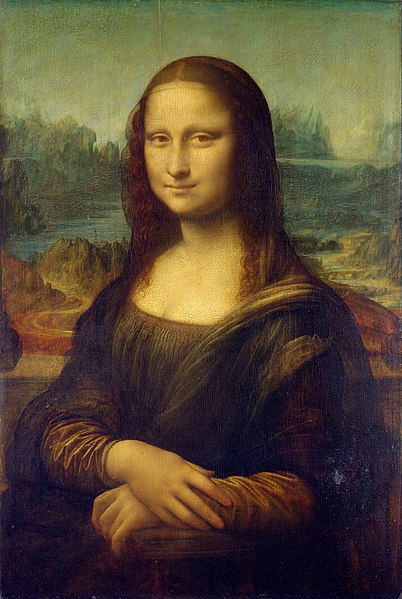
\includegraphics{monalisa}
	\caption[The Mona Lisa]{The Mona Lisa.\\ 
	\url{https://commons.wikimedia.org/wiki/File:Mona_Lisa,_by_Leonardo_da_Vinci,_from_C2RMF_retouched.jpg}}
	\labfig{marginmonalisa}
\end{marginfigure}


\setchapterpreamble[u]{\margintoc}
\chapter{A Shakespearean comedy of numbers}
\labch{intro}


This is some text and a link to 
Hey if you want to site something on the side use\sidecite{Andreu2021}

"AI Scientists disagree as to whether these language networks posess true knowledge or are just mimicking humans by remembering the statistics of millions of words. I don't beloive any kind of deep learning network will achieve the goal of AGI if the network doesn't model the world the way the brain does. Deep learning networks work well, but not because they solved the knowledge representation problem. They work well because they avoided it completely, relying on statistics and lots of data instead. How deep learning networks work is clever, their performance impressive, and they are commercially valuable. I am only pointing out that they don't possess knowledge and, therefore, are not on the path to having the ability of a five-year-old child." \cite{hawkins_2022}


\begin{lstlisting}[style=kaolstplain,linewidth=1.5\textwidth]
cd myproject
docker run tensorflow
#profit!
\end{lstlisting}

\url{tex.stackexchange.org} for help.
 
\setchapterpreamble[u]{\margintoc}
\chapter{Derivative artworks of the future?}
\labch{intro}

GPT-3, BERT and Bloom

Link some cool shit here, Draw Owl!

Who owns this shit anyway? Copilot and FSF plus lawsuits

Prove it, asshole!

I can make a "model" that behaves like a database. Just memorizes shit
 
\setchapterpreamble[u]{\margintoc}
\chapter{The data is the hardest part}
\labch{intro}

You are essentially programming with data, so if your data sucks so will your prediction, you also really can't generalize, only correllate.

are you predicting the right thing? Are you really predicting how valuable the company is or just whether it'll be the next meme stock?

“I hope for some sort of peace—but I fear that machines are ahead of morals by some centuries and when morals catch up there'll be no reason for any of it.” Harry Truman, 1945 \sidecite{McCullough1992}

Representation, "fixing the training set" \sidecite{Christian2020}, or the Impossibility of Fairness from a model.

TODO talk about these books
\cite{Oneil2017}
\cite{Perez2019}
\cite{Blackman2022Jul}
\cite{Christian2020}



"The second requirement of goal-misalignment risk is that an intelligent machine can commandeer the Earth's resources to pursue its goals, or in other ways prevent us from stopping it... We have similar concerns with humans. This is why no singer person or entity can control the entire internet and why we require multiple people to launch a nuclear missile. Intelligent machines will not develop misaligned goals unless we go to great lengths to endow them with that ability. Even if they did, no machine can commandeer the world's resources unless we let it. We don't let a single human, or even a small number of humans, control the world's resources. We need to be similarly careful with machines." \cite{hawkins_2022}

\begin{lstlisting}[style=kaolstplain,linewidth=1.5\textwidth]
cd myproject
docker run tensorflow
#profit!
\end{lstlisting}

\url{tex.stackexchange.org} for help.

 
\setchapterpreamble[u]{\margintoc}
\chapter{The police and Big Tech are profiling me!}
\labch{intro}

Classification is everywhere, it's also very useful. Just get over it. 

Online Advertising, Justice, Job Applications, Creditworthiness, Getting Insurance (Weapons of Math Destruction), Civic Life, /sidecite{Oneil2017} ; The Default Male, Invisible Women effects snow clearing schedules and drug discovery 

\begin{lstlisting}[style=kaolstplain,linewidth=1.5\textwidth]
cd myproject
docker run tensorflow
#profit!
\end{lstlisting}

\url{tex.stackexchange.org} for help.
 
\setchapterpreamble[u]{\margintoc}
\chapter{The useful chaos of spaghetti code}
\labch{intro}

Interacting Layers of Statistical Understanding
Useful Chaos

These layers are totally transparent, but you can't understand them because they're complicated, yo

You can't understand ML layers, but they are useful nonetheless.

 
\setchapterpreamble[u]{\margintoc}
\chapter{Self-stabilizing concept drift}
\labch{intro}

Many models need to constantly be retrained

Does progress slow down because we keep reusing the work of the past to generate our work?

 
\setchapterpreamble[u]{\margintoc}
\chapter{My horse drives itself, thanks!}
\labch{intro}


Can Models bring Incremental or Revolutionary Change?

Respond directly to Jon Krohn's TED talk about monkeys being dumber than us... what about construction equipmenth that's stronger than us, or racism/eugenics people that are dumber than us \sidecite{KrohnTED}

"The inhabitant of London could order by telephone, sipping his morning tea in bed, the various products of the whole earth -- he could at the same time and by the same means adventure his wealth in the natural resources and new enterprise of any quarter of the world -- he could secure forthwith, if he wished, cheap and comfortable means of transit to any country or climate without passport or other formality." - John Maynard Keynes \sidecite{Keynes2012}

Who is affected the most?

What should individuals do?

What should governments do?

What should businesses do?
 
\setchapterpreamble[u]{\margintoc}
\chapter{Skynet: did you try unplugging it?}
\labch{intro}



\appendix % From here onwards, chapters are numbered with letters, as is the appendix convention
\pagelayout{wide} % No margins
\addpart{Appendix}
\pagelayout{margin} % Restore margins

\setchapterstyle{lines}
\setchapterpreamble[u]{\margintoc}
\chapter{????}
\labch{appendix}

Let's say we want to build an ensemble model to analyze poetry, put a haiku into craiyon's online shit, then we categorize the resulting photo. \sidecite{Andreu2021}



 

%----------------------------------------------------------------------------------------

\backmatter % Denotes the end of the main document content
\setchapterstyle{plain} % Output plain chapters from this point onwards

%----------------------------------------------------------------------------------------
%	BIBLIOGRAPHY
%----------------------------------------------------------------------------------------

% The bibliography needs to be compiled with biber using your LaTeX editor, or on the command line with 'biber main' from the template directory

\defbibnote{bibnote}{Here are the references in citation order.\par\bigskip} % Prepend this text to the bibliography
\printbibliography[heading=bibintoc, title=Bibliography, prenote=bibnote] % Add the bibliography heading to the ToC, set the title of the bibliography and output the bibliography note

%----------------------------------------------------------------------------------------
%	NOMENCLATURE
%----------------------------------------------------------------------------------------

% The nomenclature needs to be compiled on the command line with 'makeindex main.nlo -s nomencl.ist -o main.nls' from the template directory

\nomenclature{$c$}{Speed of light in a vacuum inertial frame}
\nomenclature{$h$}{Planck constant}

\renewcommand{\nomname}{Notation} % Rename the default 'Nomenclature'
\renewcommand{\nompreamble}{The next list describes several symbols that will be later used within the body of the document.} % Prepend this text to the nomenclature

\printnomenclature % Output the nomenclature

%----------------------------------------------------------------------------------------
%	GLOSSARY
%----------------------------------------------------------------------------------------

% The glossary needs to be compiled on the command line with 'makeglossaries main' from the template directory

\setglossarystyle{listgroup} % Set the style of the glossary (see https://en.wikibooks.org/wiki/LaTeX/Glossary for a reference)
\printglossary[title=Special Terms, toctitle=List of Terms] % Output the glossary, 'title' is the chapter heading for the glossary, toctitle is the table of contents heading

%----------------------------------------------------------------------------------------
%	INDEX
%----------------------------------------------------------------------------------------

% The index needs to be compiled on the command line with 'makeindex main' from the template directory

\printindex % Output the index

%----------------------------------------------------------------------------------------
%	BACK COVER
%----------------------------------------------------------------------------------------

% If you have a PDF/image file that you want to use as a back cover, uncomment the following lines

%\clearpage
%\thispagestyle{empty}
%\null%
%\clearpage
%\includepdf{cover-back.pdf}

%----------------------------------------------------------------------------------------

\end{document}
